%Template file for a presentation using Latex and beamer
%You will need to install Latex, the beamer package, and some of these other packages on your own.
\documentclass[11pt,compress]{beamer} %slides and notes
\usepackage{amsmath,datetime,array,alltt,graphicx,xmpmulti,mathtools,bbm,booktabs,xspace,mathabx,tikz,pifont,epstopdf,relsize,wedn,hyperref,framed}
\usepackage[justification=centering]{caption}
\usepackage{subcaption}\captionsetup{compatibility=false}
\usepackage[autolinebreaks]{mcodefred}
\usepackage[author-year]{amsrefs}
\usepackage{qtree}
\usepackage{pst-node}% http://ctan.org/pkg/pst-node
\usepackage{textcomp} %helps to compile MATLAB code in mcode or lstlisting
\usepackage{pgf,pgfarrows,pgfnodes} % Drawing tables, arrows, ...
\usepackage[customcolors]{hf-tikz} % Box equations
\input FJHDef.tex


\newcommand{\HickernellFJ}{Hickernell} %To give my name to the bibliography

\newtheorem{lem}{Lemma}
\setbeamertemplate{theorems}[numbered]

\usetikzlibrary{arrows}
\newcommand*\circled[1]{\tikz[baseline=(char.base)]{
  \node[shape=circle,color=green,draw,inner sep=1pt] (char) {#1};}}
\setlength{\parskip}{2ex}
\setlength{\arraycolsep}{0.5ex}
\newcommand{\tol}{\text{tol}}
\newcommand{\e}{\text{e}}
\DeclareMathOperator{\cubMC}{cubMC}
\DeclareMathOperator{\qse}{qse}
\DeclareMathOperator{\integ}{int}
\DeclareMathOperator{\trap}{trap}
\DeclareMathOperator{\size}{size}
\DeclareMathOperator{\app}{id}
\DeclareMathOperator{\err}{err}
\DeclareMathOperator{\walsh}{walsh}
\newcommand{\happ}{\widehat{\app}}
\newcommand{\hinteg}{\widehat{\integ}}
\newcommand{\cube}{[0,1)^d}
\newcommand{\desall}{\{\vx_i\}}
\newcommand{\desn}{\{\vz_i\}_{i=0}^{n-1}}
\def\newblock{\hskip .11em plus .33em minus .07em}
\newcommand{\wcS}{\widecheck{S}}
\newcommand{\wcomega}{\widecheck{\omega}}
\newcommand{\prob}[1]{\mathbb{P}\left( #1 \right)}
\newcommand{\bsk}{\boldsymbol{k}}    % vector k
\newcommand{\bsz}{\boldsymbol{z}}    % vector z
\newcommand{\bsx}{\boldsymbol{x}}    % vector z
\newcommand{\F}{\mathbb{F}} % field, finite field
\newcommand{\bsDelta}{\boldsymbol{\Delta}}    % vector
\newcommand{\bszero}{\boldsymbol{0}} % vector of zeros
\newcommand{\E}{{\rm e}}
\newcommand{\D}{{\rm d}}
\newcommand{\Z}{\mathbb{Z}}
\newcommand{\R}{\mathbb{R}}
\newcommand{\N}{\mathbb{N}}
\newcommand{\I}{\mathsf{I}}
\DeclareMathOperator{\Var}{Var}
\DeclareMathOperator{\affine}{affine}
\DeclareMathOperator{\Genz}{Genz}
\DeclareMathOperator{\payoff}{payoff}
\newcommand{\intalg}{\hI\left(\vx\mapsto f(\vx),\varepsilon_a\right)}

\definecolor{orange_plot}{rgb}{1.,.5,.0}
\definecolor{gray_plot}{rgb}{.7,.7,.7}
\definecolor{green_plot}{rgb}{.0,.5,.0}


\usetheme{FredIIT}
% \usetheme{Berlin}
\logo{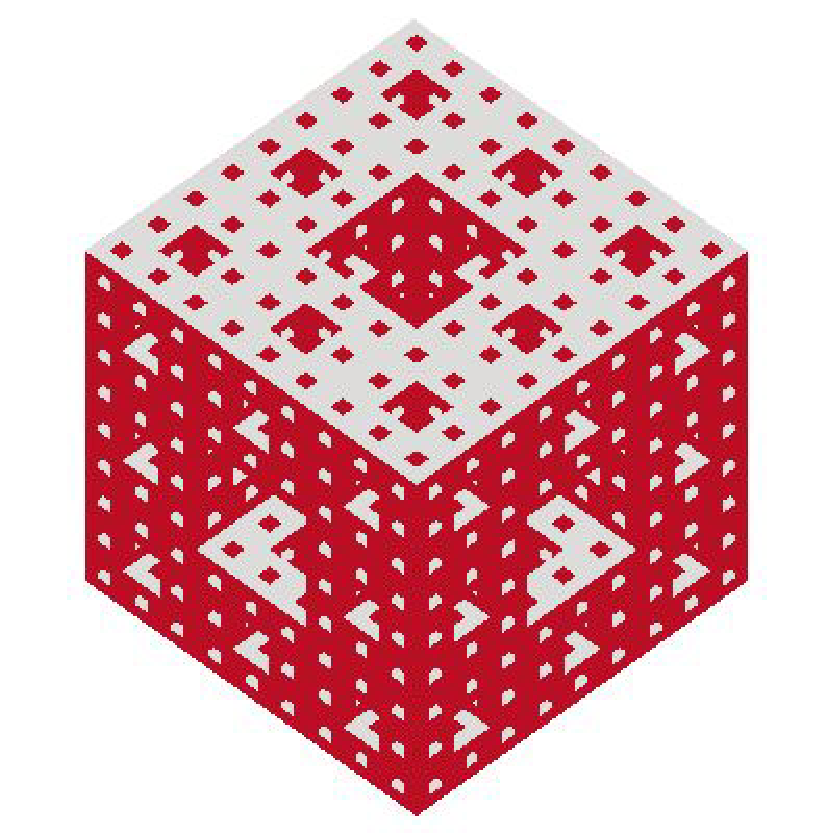
\includegraphics[width=1cm]{MengerIITRedGray.pdf}}

\title[CASSC 2016]{Minimizing the Number of Function Evaluations to Estimate Sobol' Indices}
\author[ljimene1@hawk.iit.edu]{Llu\'is Antoni Jim\'enez Rugama\\Joint work with: Fred J. Hickernell (IIT),\\Cl\'ementine Prieur (Univ. Grenoble), Elise Arnaud (Univ. Grenoble), Herv\'{e} Monod (INRA), and Laurent Gilquin (Univ. Grenoble)}
\institute{Room 120, Bldg E1, Department of Applied Mathematics \\
Illinois Institute of Technology, Chicago, 60616 IL \\
Email: \href{mailto:ljimene1@hawk.iit.edu}{\url{ljimene1@hawk.iit.edu}}}
%Website: \url{http://math.iit.edu/~lantoni/}
% \date[{Revised \currenttime, \mdyyyydate \today}]{Revised \settimeformat{ampmtime} \currenttime, \today}
\date[]{\today}
%{Monday ${\rm{28^{th}}}$ September, 2015}

\begin{document}
\frame{\titlepage}

%\frame{\frametitle{Outline}\begin{minipage}{15cm}\tableofcontents\end{minipage}}
%\AtBeginSection[]
%{ \begin{frame}
%  \frametitle{Outline}
%  \begin{minipage}{15cm}
%  \tableofcontents[currentsection]
%  \end{minipage}
%  \end{frame}
%}

\begin{frame}<1>[label = Outline]\frametitle{Outline}
\begin{itemize}
\item<1,2> \alert<2>{Introduction}\only<2>{---The ANalysis Of VAriance.}
\item<1,3> \alert<3>{Sobol' Indices}\only<3>{---Measuring the importance of each input.}
\item<1,4> \alert<4>{Replicated Method}\only<4>{---Reducing the number of function evaluations to compute \emph{first-order} indices.}
\item<1,5> \alert<5>{Quasi-Monte Carlo Methods}\only<5>{---How can we construct replicated quasi-Monte Carlo sequences?}
\end{itemize}
\end{frame}

\section{Introduction}
\setbeamercovered{transparent} % Translucid <only>
\againframe<2>{Outline}
\setbeamercovered{invisible} % Invisible <only>

\begin{frame}
\frametitle{The Noisy Students}
Consider three noisy students in my class:
\begin{columns}
  \begin{column}{.45\textwidth}
  \center
  \vspace{-.5cm}
	\begin{equation*}
	\tikzmarkin{a}(0.2,-0.5)(-0.2,1.25)
	\overbrace{f(U_1,U_2,U_3)=\e^{3/2U_1+U_2}+\cos(2\pi U_3)}^{\text{Noise Model}}
	\tikzmarkend{a}
	\end{equation*}
  \end{column}
  \begin{column}{.45\textwidth}
  \center
    
\includegraphics[width=.75\textwidth]{minions.jpg}
  	\[U_1,U_2,U_3 \text{ IID}\sim U([0,1])\]
  \end{column}
\end{columns}

\end{frame}

\begin{frame}
\frametitle{ANOVA}
For $f\in L^2\left([0,1]^d\right)$, and $\mathcal{D}=\{1,\dots,d\}$,
\begin{equation*}
f(\vx)=\sum \limits_{u \subseteq \mathcal{D}} f_u(\vx)\, , \qquad f_{\varnothing} = \mu\, ,
\label{anova}
\end{equation*}
where,
\[f_u(\vx)= \int_{[0,1]^{d-|u|}} f(\vx) d{\vx}_{-u} - \sum \limits_{v \subset u} f_v(\vx)\, .\]

\begin{itemize}
\item $\abs{u}$ the cardinality of $u$.
\item $-u:=u^c=\mathcal{D}\setminus u$.
\end{itemize}
\end{frame}

\begin{frame}
\frametitle{Variance Decomposition}
Under the previous definitions,
\begin{equation*}
\sigma^2_{\varnothing} = 0\, ,\qquad \sigma^2_{u} =\int_{[0,1]^{d}} f_u(\vx)^2 d{\vx}\, ,\qquad \sigma^2 =\int_{[0,1]^{d}} \left(f(\vx)-\mu\right)^2 d{\vx}\, .
\end{equation*}
The ANOVA identity is,

\[
\sigma^2 = \sum \limits_{u \subseteq\mathcal{D}} \sigma_u^2 \, .
\]
\end{frame}

\section{Sobol Indices'}
\setbeamercovered{transparent} % Translucid <only>
\againframe<3>{Outline}
\setbeamercovered{invisible} % Invisible <only>

\begin{frame}
\frametitle{Sobol' Indices}
We consider $f(\vx)$ as a random variable with $\vx\sim U\left([0,1)^d\right)$.

Sobol' introduced the \emph{global sensitivity} indices which measure the variance explained by any dimension subset $u\in\mathcal{D}$:
\begin{equation*}
\underline{\tau}_u^2 = \sum_{\substack{v \subseteq u \\ v\,\in\mathcal{D}}} \sigma_v^2\, , \quad \text{ and } \quad \overline{\tau}_u^2 = \sum_{\substack{v \cap u\neq\varnothing \\ v\,\in\mathcal{D}}} \sigma_v^2\, .
\end{equation*}
We have the following properties,
\begin{itemize}
\item $\underline{\tau}_u^2\leq \overline{\tau}_u^2$.
\item $\underline{\tau}_u^2 + \overline{\tau}_{-u}^2 =\sigma^2$.
\end{itemize}
\end{frame}

\begin{frame}
\frametitle{The Noisy Students Are Back!}
\centering

\includegraphics[width=.55\textwidth]{minions.jpg}

\begin{tabular}{ll|c|r}
\hspace{-1.5cm} & $u=\{1\}$ & $u=\{2\}$ & $u=\{3\}$ \\
\hline
\hspace{-1.5cm}$\underline{\tau}_u^2/\sigma^2$: & 58.5\% & 26.5\% & 10.2\% \\
\hspace{-1.5cm}$\overline{\tau}_{u}^2/\sigma^2$: & 63.3\% & 31.3\% & 10.2\%
\end{tabular}
\end{frame}

\begin{frame}
\frametitle{Normalized \emph{First-Order} Sobol' Indices}
In this particular case, we consider $\abs{u}=1$ and want to estimate $\underline{\tau}_u^2/\sigma^2=\sigma_u^2/\sigma^2$. For this purpose, given $\vx,\vx'\in [0,1]^d$, we define the following point,
\begin{gather*}
(\vx_u:{\color{blue}\vx'_{-u}}) := ({\color{blue}x'_1},\dots,{\color{blue}x'_{u-1}},x_u,{\color{blue}x'_{u+1}},\dots,{\color{blue}x'_d})\in [0,1]^d.
\end{gather*}

Thus, one can use the following integral form to build an estimator:
\begin{equation*}
\frac{\sigma_u^2}{\sigma^2}=\frac{\int_{[0,1)^{2d-1}}(\overbrace{f(\vx)}^{g(\vx,\vx'):=} - \mu) (\overbrace{f(\vx_u:{\vx'}_{-u})}^{g_u(\vx,\vx'):=}-\mu) d\vx d{\vx'}_{-u}}{\int_{[0,1]^d} f(\vx)^2 d{\vx}-\mu^2}=H(g,g_u)\, .
\end{equation*}
\end{frame}

%\begin{frame}
%\frametitle{Sobol' Indices}
%For $\vX\sim U[0,1]^d$, we are interested in estimating the \emph{first-order} and \emph{total-effect} normalized indices,
%\setbeamercovered{transparent} % Translucid <only>
%\begin{gather*}
%\underline{\tau}_u^{2,*}=\frac{\Var \left[ \mathbb{E} \left(f({\vX})|{\vX}_{u}\right)\right] }{\Var\left(f({\vX})\right)}\uncover<1>{=
%1-\frac{\mathbb{E}\left[ \Var \left(f({\vX})|\vX_u\right)\right]}{\Var\left(f({\vX})\right)},}\\
%\uncover<1>{\overline{\tau}_u^{2,*}=1-\frac{\Var \left[ \mathbb{E} \left(f({\vX})|\vX_{-u}\right)\right]}{\Var\left(f({\vX})\right)}=\frac{\mathbb{E}\left[ \Var \left(f({\vX})|{\vX}_{-u}\right)\right] }{\Var\left(f({\vX})\right)}.}
%\end{gather*}
%satisfying $
%0\leq \underline{\tau}_u^{2,*} \leq \overline{\tau}_u^{2,*}\leq 1$.\setbeamercovered{invisible} % Invisible <only>
%\vspace{-0.2cm}
%\uncover<2>{The \emph{first-order} indice is composed by,
%\begin{equation*}
%\underline{\tau}_u^{2,*}=\frac{I^{(1)}}{I^{(2)}-\left(I^{(3)}\right)^2},\quad \text{where }\begin{cases}I^{(1)}\text{ is a }2d-1\text{ dim. integral.} \\ I^{(2)}\text{ is a }d\text{ dim. integral.} \\ I^{(3)}\text{ is a }d\text{ dim. integral.} \end{cases}
%\end{equation*}
%%\vspace{-0.3cm}
%Error bounds for $\underline{\tau}_u^2$ require more care than error bounds for $I^{(k)}$.
%}
%\end{frame}

\begin{frame}
\frametitle{Numerical Integration Problem}
We will focus on reducing the number of function evaluations, and to estimate $\sigma_u^2/\sigma^2$, only $g$ and $g_u$ are evaluated.

Computing all the indices one by one, if one requires $n$ points for each estimation, the total number of function evaluations of $g$ and $g_u$ are
\[
2dn\, ,
\]
However, if all indices are computed together, $g$ only needs to be evaluated once. Therefore, the number of function evaluations becomes
\[
(1+d)n\, ,
\]
Finally, under a special set of quasi-Monte Carlo sequences, this number is decreased to
\[
2n\, .
\]
\end{frame}

\section{Replicated Method}
\setbeamercovered{transparent} % Translucid <only>
\againframe<4>{Outline}
\setbeamercovered{invisible} % Invisible <only>

\begin{frame}
\frametitle{Replicated points}
Functions $g$ and $g_u$ only share input dimension $u$:
\begin{gather*}
g(\vx,{\color{blue}\vx'})=f(x_1,\dots,x_{u-1},x_u,x_{u+1},\dots,x_d)\, ,\\
g_u(\vx,{\color{blue}\vx'})=f({\color{blue}x'_1},\dots,{\color{blue}x'_{u-1}},x_u,{\color{blue}x'_{u+1}},\dots,{\color{blue}x'_d})\, .
\end{gather*}
Hence, we can construct our points $\vx'_i$ as follows,
\begin{equation*}
\begin{pmatrix}
x_{0,1} & \cdots & x_{0,d} \\
\vdots & \ddots & \vdots \\
x_{n,1} & \cdots & x_{n,d} \\
\vdots &  & \vdots
\end{pmatrix},\qquad
\begin{pmatrix}
{\color{blue}x'_{0,1}} & \cdots & {\color{blue}x'_{0,d}} \\
\vdots & \ddots & \vdots \\
{\color{blue}x'_{n,1}} & \cdots & {\color{blue}x'_{n,d}} \\
\vdots &  & \vdots
\end{pmatrix}=
\begin{pmatrix}
x_{{\color{blue}\pi_1(0)},1} & \cdots & x_{{\color{blue}\pi_d(0)},d} \\
\vdots & \ddots & \vdots \\
x_{{\color{blue}\pi_1(n)},1} & \cdots & x_{{\color{blue}\pi_d(n)},d} \\
\vdots &  & \vdots \\
\end{pmatrix}\, .
\end{equation*}
\end{frame}

\begin{frame}
\frametitle{The Right Function Values}
\only<1>{
Given the right order of points:
\begin{equation*}
\begin{pmatrix}
{\color{blue}\vx'_{\pi^{-1}_u(0)}} \\
\vdots \\
{\color{blue}\vx'_{\pi^{-1}_u(n)}} \\
\vdots
\end{pmatrix}=
\begin{pmatrix}
{\color{blue}x'_{\pi^{-1}_u(0),1}} & \cdots & {x_{0,u}} & \cdots & {\color{blue}x'_{\pi^{-1}_u(0),d}} \\
\vdots & & \vdots & & \vdots \\
{\color{blue}x'_{\pi^{-1}_u(n),1}} & \cdots & x_{n,u} & \cdots & {\color{blue}x'_{\pi^{-1}_u(n),d}} \\
\vdots & & \vdots & & \vdots
\end{pmatrix}\, .
\end{equation*}}
\only<2>{
We only need to evaluate $g_u(\vx,\vx')$ once:
\begin{equation*}
\begin{pmatrix}
f({\color{blue}\vx'_{0}}) \\
\vdots \\
f({\color{blue}\vx'_{n}}) \\
\vdots
\end{pmatrix}=
\begin{pmatrix}
y_{0} \\
\vdots \\
y_{n} \\
\vdots
\end{pmatrix} \Longrightarrow
\begin{pmatrix}
g_u(\vx_0,{\color{blue}\vx'_0})\\
\vdots\\
g_u(\vx_n,{\color{blue}\vx'_n})\\
\vdots\\
\end{pmatrix}=
\begin{pmatrix}
y_{\pi^{-1}_u(0)} \\
\vdots \\
y_{\pi^{-1}_u(n)} \\
\vdots
\end{pmatrix}
\end{equation*}
}
\end{frame}

\section{Quasi-Monte Carlo Methods}
\setbeamercovered{transparent} % Translucid <only>
\againframe<5>{Outline}
\setbeamercovered{invisible} % Invisible <only>

\begin{frame}
\frametitle{Quasi-Monte Carlo Sequences}
\only<1>{
For $i\in\mathbb{N}_0$ and $x\in [0,1)$,
\[
i = \sum_{k\geq 0}i_kb^{k}\, , \qquad x = \sum_{k\geq 1}x_kb^{-k}\, , \qquad i_k,x_k\in\mathbb{F}_b .
\]
Each dimension $j$ of a digital net is constructed according to:
\[
\begin{pmatrix}
x_1 \\ \vdots \\ x_m \\ \vdots
\end{pmatrix}=
C_j
\begin{pmatrix}
i_0 \\ \vdots \\ i_{m-1} \\ \vdots
\end{pmatrix}\, , \qquad C_j\in M^{\infty\times\infty}(\mathbb{F}_b)\, .
\]}
\only<2>{
For instance, the $5$th point of a Sobol' sequence in base 2 and dimension $3$:
\[
\left(
C_1 \begin{pmatrix}
1 \\ 0 \\ 1 \\ 0 \\ \vdots
\end{pmatrix},
C_2 \begin{pmatrix}
1 \\ 0 \\ 1 \\ 0 \\ \vdots
\end{pmatrix},
C_3 \begin{pmatrix}
1 \\ 0 \\ 1 \\ 0 \\ \vdots
\end{pmatrix}
\right) =
\left(
\begin{pmatrix}
1 \\ 0 \\ 1 \\ 0 \\ \vdots
\end{pmatrix},
\begin{pmatrix}
0 \\ 0 \\ 1 \\ 0 \\ \vdots
\end{pmatrix},
\begin{pmatrix}
1 \\ 1 \\ 1 \\ 0 \\ \vdots
\end{pmatrix}
\right)
\begin{matrix}
\leftarrow 1/2 \\ \leftarrow 1/4 \\ \leftarrow 1/8 \\ \hspace{.2cm}\leftarrow 1/16 \\ \hspace{.2cm}\vdots
\end{matrix}
\]
\[
\vx_5 = (0.625\, ,0.125\, ,0.875).
\]
}
\only<3>{
For the Sobol' sequences, we can for instance, construct our permutations through an upper triangular matrix $U\in M^{\infty\times\infty}(\mathbb{F}_b)$ applied as follows,
\[
\begin{pmatrix}
x_1 \\ \vdots \\ x_m \\ \vdots
\end{pmatrix}=
C_j U
\begin{pmatrix}
i_0 \\ \vdots \\ i_{m-1} \\ \vdots
\end{pmatrix}.
\]
}
\end{frame}

\begin{frame}
\frametitle{Conclusions}
\begin{itemize}
\item We can study how each \alert{dimension explains the overall variance} of a model using \alert{Sobol' Indices}.
\item \alert{\emph{First-order} Sobol' Indices} can be estimated using \alert{only $2n$} function evaluations (not depending on $d$).
\item Our \alert{quasi-Monte Carlo automatic cubatures} can be adapted to estimate these indices adaptively.
\end{itemize}
\end{frame}

\part{References}
\begin{frame}[allowframebreaks]\frametitle{References}
\nocite{Owen2013VCG,Sobol01Global,Owe98b,HicJim16a,Nie92}
\bibliography{FJHown23,FJH22,lluisantoni}
\end{frame}


\end{document}
